\chapter{Parallel transport}
\label{chap:parallel-transport}

\section{Parallel tangent fields}

Let $\Sigma$ be a smooth surface and $\gamma\:[a,b]\z\to \Sigma$ be a smooth curve.
A smooth vector-valued function $t\mapsto {\vec v}(t) \in \mathbb{R}^3$ is called a \index{tangent!field}\emph{tangent field} along $\gamma$ if
the vector ${\vec v}(t)$ lies in the tangent plane $\T_{\gamma(t)}\Sigma$ for each~$t$.

A tangent field $\vec v$ on $\gamma$ is called \index{parallel!field}\emph{parallel} if ${\vec v}'(t)\perp\T_{\gamma(t)}$ for any~$t$.

In general, the family of tangent planes $\T_{\gamma(t)}\Sigma$ is not parallel.
Therefore, one cannot expect to have a \textit{truly} parallel field with ${\vec v}'(t)\equiv 0$.
The condition ${\vec v}'(t)\perp\T_{\gamma(t)}$ means that the family is \textit{as parallel as possible} --- it rotates together with the tangent plane but does not rotate inside the plane.

By the definition of geodesic, the velocity field ${\vec v}(t)\z=\gamma'(t)$ of any geodesic $\gamma$ is parallel on~$\gamma$.

\begin{thm}{Exercise}\label{ex:parallel}
Let $\Sigma$ be a smooth surface and let 
$\gamma\:[a,b]\to \Sigma$ be a smooth curve.
Suppose ${\vec v}(t)$, $\vec w(t)$ are parallel vector fields along~$\gamma$.

\begin{subthm}{ex:parallel:a} Show that $|{\vec v}(t)|$ is constant.
\end{subthm}

\begin{subthm}{ex:parallel:b} Show that the angle $\theta(t)=\measuredangle({\vec v}(t),\vec w(t))$ is constant.
\end{subthm}

\end{thm}

\section{Parallel transport}

\begin{thm}{Proposition-Definition}\label{prop:parallel}
Let $\gamma\:[a,b]\z\to \Sigma$ be a piecewise smooth curve on a smooth surface $\Sigma$.
Assume $p=\gamma(a)$ and $q=\gamma(b)$.

Given a tangent vector ${\vec w}\in\T_p$ there is a unique parallel field ${\vec w}(t)$ along $\gamma$ such that ${\vec w}(a)={\vec w}$.

The vector ${\vec w}(b)\in\T_q$ is called the \index{parallel!transport}\emph{parallel transport} of ${\vec w}(a)$ along~$\gamma$ in~$\Sigma$.
\end{thm}



The parallel transport along $\gamma$ will be denoted by $\iota_\gamma$;
so we can write $\vec w(b)=\iota_\gamma({\vec w}(a))$ or $\vec w(b)=\iota_\gamma({\vec w}(a))_\Sigma$ if we need to emphasize that $\gamma$ lies on the surface~$\Sigma$.
From Exercise~\ref{ex:parallel}, it follows that parallel transport $\iota_\gamma\:\T_p\z\to\T_q$ is an isometry.
In general, the parallel transport $\iota_\gamma\:\T_p\z\to\T_q$ depends on the choice of $\gamma$; that is, for another curve $\gamma_1$ connecting $p$ to $q$ in $\Sigma$, the parallel transports $\iota_{\gamma_1}$ and $\iota_{\gamma}$ might be different.

\parbf{Sketch of proof.}
Assume $\gamma$ is smooth and lies in a local chart $(u,v)\z\mapsto s(u,v)$ of $\Sigma$;
so $\gamma(t)\z=s(u(t),v(t))$ for smooth functions $t\mapsto u(t)$ and $t\mapsto v(t)$.
Set 
\[
\vec u(t)=s_u(u(t),v(t)),
\quad
\vec v(t)=s_v(u(t),v(t)),
\quad
\text{and}
\quad
\Norm(t)=\Norm(\gamma(t)).
\]

The conditions $\vec w(t)\in \T_{\gamma(t)}$ and $\vec w'(t)\perp \T_{\gamma(t)}$ can be written as a system of equations:
\[
\begin{cases}
\ \langle\vec w(t), \Norm(t)\rangle=0,
\\
\ \langle\vec w'(t), \vec u(t)\rangle=0,
\\
\ \langle\vec w'(t), \vec v(t)\rangle=0.
\end{cases}
\]
Rewriting this system in components of $\vec u$, $\vec v$, $\vec w$, and $\Norm$ produces a system of ordinary differential equations on the components of $\vec w$.
Applying \ref{thm:ODE}, we get a solution $\vec w(t)$.
By \ref{ex:parallel}, $|\vec w|$ is constant;
therefore \ref{thm:ODE} implies that $\vec w$ is defined on the whole interval $[a,b]$.

If $\gamma$ is only piecewise smooth or not covered by one chart we can subdivide it into smooth arcs $\gamma_1,\dots,\gamma_n$ such that each $\gamma_i$ lies in one chart.
Applying the statement consecutively to each $\gamma_i$ proves it for $\gamma$.
\qeds

Suppose $\gamma_1$ and $\gamma_2$ are two smooth curves in two smooth surfaces $\Sigma_1$ and $\Sigma_2$.
Denote by $\Norm_i\:\Sigma_i\to\mathbb{S}^2$ the Gauss maps of $\Sigma_1$ and $\Sigma_2$.
If $\Norm_1\circ\gamma_1(t)= \Norm_2\circ\gamma_2(t)$ for any $t$, then we say that the curves $\gamma_1$ and $\gamma_2$ have {}\emph{identical normals} in $\Sigma_1$ and $\Sigma_2$, respectively.

In this case, the tangent plane $\T_{\gamma_1(t)}\Sigma_1$ is parallel to $\T_{\gamma_2(t)}\Sigma_2$ for any~$t$.
Therefore we can identify $\T_{\gamma_1(t)}\Sigma_1$ with $\T_{\gamma_2(t)}\Sigma_2$.
In particular, if $\vec v(t)$ is a tangent vector field along $\gamma_1$,
then it is also a tangent vector field along $\gamma_2$.
Moreover, $\vec v'(t)\perp \T_{\gamma_1(t)}\Sigma_1$ is equivalent to $\vec v'(t)\perp \T_{\gamma_2(t)}\Sigma_2$; that is, if $\vec v(t)$ is parallel along $\gamma_1$,
then it is also parallel along $\gamma_2$.

The discussion above leads to the following observation that will play a key role in the sequel.

\begin{thm}{Observation}\label{obs:parallel=}
Let $\gamma_1$ and $\gamma_2$ be two smooth curves in two smooth surfaces $\Sigma_1$ and $\Sigma_2$.
Suppose $\gamma_1$ and $\gamma_2$ have identical normals (as the curves in $\Sigma_1$ and $\Sigma_2$, respectively).
Then the parallel transports $\iota_{\gamma_1}$ and $\iota_{\gamma_2}$ are identical. 
\end{thm}

\begin{thm}{Exercise}\label{ex:parallel-transport-support}
Let $\Sigma_1$ and $\Sigma_2$ be two surfaces with a common curve~$\gamma$.
Suppose $\Sigma_1$ bounds a region that contains $\Sigma_2$.
Show that the parallel translation along $\gamma$ in $\Sigma_1$ 
coincides with the parallel translation along $\gamma$ in $\Sigma_2$. 
\end{thm}

\section{Bike wheel and projections}

Here we give two interpretations of parallel transport;
they might help to build the right intuition, but will not help in writing rigorous proofs.
The first is an experiment with a bike wheel suggested by Mark Levi \cite{levi}.
The second one uses orthogonal projections of tangent planes.

Suppose $\gamma\:[a,b]\to\Sigma$ is a smooth arc in a smooth surface $\Sigma$.
Think of walking along $\gamma$ and carrying a perfectly balanced bike wheel so that you keep the wheel's axis normal to $\Sigma$ and touch only its axis.
If the wheel is not spinning at the starting point $p=\gamma(a)$, then it will not be spinning after stopping at~$q=\gamma(b)$.
Indeed, by pushing the axis one cannot produce torque to spin the wheel.
Then the map that sends the initial position of the wheel to the final position is the parallel transport~$\iota_\gamma$.

\begin{figure}[ht!]
\vskip-0mm
\centering
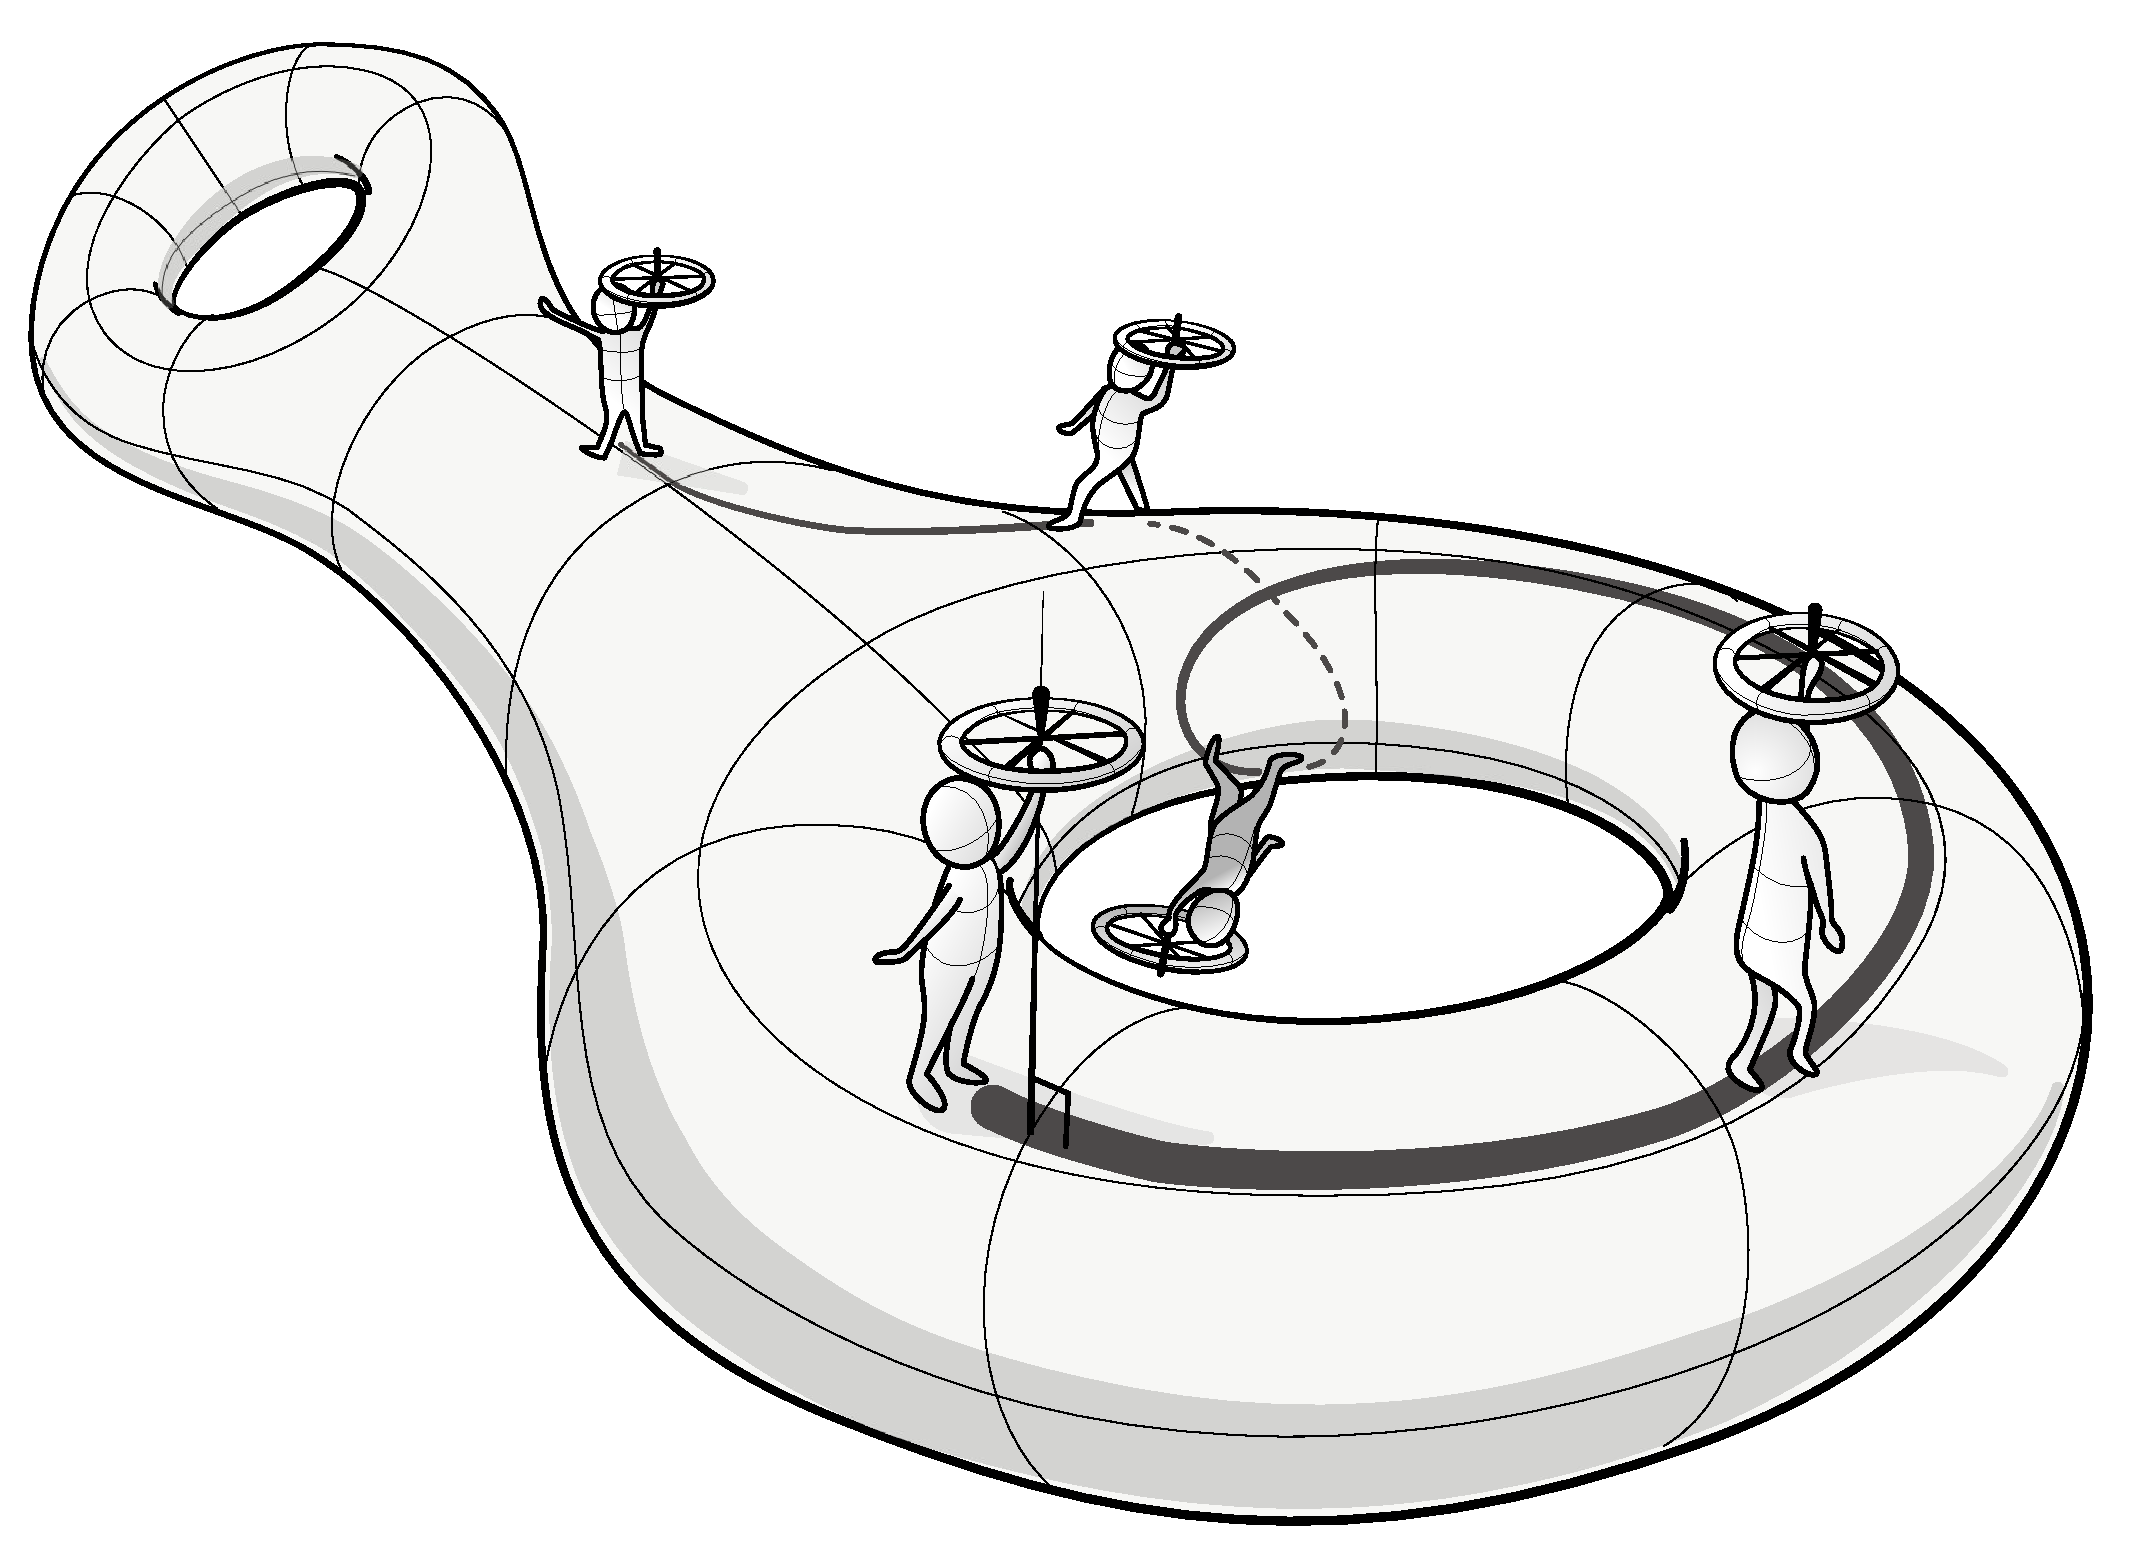
\includegraphics[scale=.3]{pics/parallel_transport}
\end{figure}

By the way, physical intuition should tell you that \textit{moving the axis of the wheel without changing its direction does not change the direction of the wheel's spokes};
this is essentially the statement of Observation~\ref{obs:parallel=}.

On a more formal level, one can choose a partition $a=t_0<\dots\z<t_n=b$ of $[a,b]$
and consider the sequence of orthogonal projections $\phi_i\:\T_{\gamma(t_{i-1})}\to\T_{\gamma(t_i)}$.
For a fine partition, the composition 
\[\phi_n\circ\dots\circ\phi_1\:\T_p\z\to\T_q\]
gives an approximation of $\iota_\gamma$.

Each $\phi_i$ does not increase the magnitude of a vector and neither the composition.
It is straightforward to see that if the partition is sufficiently fine, then the above composition is almost an isometry.
Therefore, the limit $\iota_\gamma$ is an isometry $\T_p\z\to\T_q$.

\begin{thm}{Exercise}\label{ex:holonomy=not0}
Construct a loop $\gamma$ in $\mathbb{S}^2$ such that the parallel transport $\iota_\gamma$ is not the identity map.
\end{thm}

\section{Total geodesic curvature}

Recall that geodesic curvature is defined in Section~\ref{sec:Darboux}.
It is denoted by $k_g$, and it measures how much a curve $\gamma$ on an oriented surface diverges from being a geodesic;
it is positive where $\gamma$ turns left and negative where $\gamma$ turns right.
In particular, geodesics have vanishing geodesic curvature.

Suppose $\Sigma$ is a smooth oriented surface, and $\gamma\:\mathbb{I}\to \Sigma$ is a smooth unit-speed curve.
The total geodesic curvature of $\gamma$ is defined by the integral 
\[\tgc\gamma
\df
\int_{\mathbb{I}} k_g(t)\cdot dt.\]

If $\Sigma$ is a plane, then the geodesic curvature of $\gamma$ coincides
with its signed curvature (see Section~\ref{sec:Total signed curvature}). 
In particular, its total geodesic curvature is equal to its total signed curvature.
For that reason, we use the same notation $\tgc\gamma$; if we need to emphasize that we consider $\gamma$ as a curve in $\Sigma$, we write $\tgc\gamma_\Sigma$.\index{10psi@$\tgc\gamma$, $\tgc\gamma_\Sigma$ (total geodesic curvature)}

If $\gamma$ is a piecewise smooth curve in $\Sigma$, then
its \index{total!geodesic curvature}\emph{total geodesic curvature} is defined as the sum of all total geodesic curvatures of its arcs plus the sum of the signed exterior angles of $\gamma$ at the joints.
More precisely, if $\gamma$ is a concatenation of smooth curves $\gamma_1,\dots,\gamma_n$, then
\[\tgc\gamma
\df
\tgc{\gamma_1}+\dots+\tgc{\gamma_n}+\theta_1+\dots+\theta_{n-1},\]
where $\theta_i$ is the signed external angle at the joint between $\gamma_i$ and $\gamma_{i+1}$;
it is positive if $\gamma$ turns left and negative if $\gamma$ turns right, it is undefined if $\gamma$ turns to the opposite direction.
If $\gamma$ is closed, then 
\[\tgc\gamma
\df
\tgc{\gamma_1}+\dots+\tgc{\gamma_n}+\theta_1+\dots+\theta_n,\]
where $\theta_n$ is the signed external angle at the joint $\gamma_n$ and $\gamma_1$.

If each arc $\gamma_i$ in the concatenation is a minimizing geodesic, then $\gamma$ is called a \index{broken geodesic}\emph{broken geodesic}.
In this case, $\tgc{\gamma_i}=0$ for each~$i$.
Therefore the total geodesic curvature of $\gamma$ is the sum of its signed external angles.

\begin{thm}{Proposition}\label{prop:pt+tgc}
Assume $\gamma$ is a closed broken geodesic in a smooth oriented surface $\Sigma$ that starts and ends at the point~$p$.
Then the parallel transport $\iota_\gamma\:\T_p\to\T_p$ is a clockwise rotation of the plane $\T_p$ by the angle~$\tgc\gamma$.

Moreover, the same statement holds true for smooth closed curves and piecewise smooth curves.
\end{thm}

\parbf{Proof.}
Assume $\gamma$ is a cyclic concatenation of geodesics $\gamma_1,\dots,\gamma_n$.
Fix a tangent vector ${\vec v}$ at $p$, and extend it to a parallel vector field along~$\gamma$.
Since $\tan_i(t)=\gamma_i'(t)$ is parallel along $\gamma_i$, the oriented angle $\phi_i$ from $\tan_i$ to ${\vec v}$ stays constant along each~$\gamma_i$.

\begin{wrapfigure}{o}{22 mm}
\vskip-0mm
\centering
\includegraphics{mppics/pic-48}
\vskip4mm
\end{wrapfigure}

Suppose $\theta_i$ denotes the external angle at the joint between $\gamma_{i}$ and $\gamma_{i+1}$.
Then 
\[\phi_{i+1}=\phi_i-\theta_i \pmod{2\cdot\pi}.\]
Therefore, after going over all vertices we get that 
\[\phi_{n+1}-\phi_1=-\theta_1-\dots-\theta_n=-\tgc\gamma \pmod{2\cdot\pi}.\]
Hence, the first statement follows.

For a smooth unit-speed curve $\gamma\:[a,b]\to\Sigma$, the proof is analogous.
Denote by $\phi(t)$ is the signed angle from $\tan (t)$ to ${\vec v} (t)$.
Let us show that 
\[\phi'(t)+k_g(t)\equiv0\eqlbl{eq:phi'+kg}\]

Recall that $\mu=\mu(t)$ denotes the counterclockwise rotation of $\tan \z=\tan(t)$ by angle $\tfrac\pi2$ in $\T_{\gamma(t)}$.
Denote by $\vec w=\vec w(t)$ the counterclockwise rotation of $\vec v=\vec v(t)$ by angle $\tfrac\pi2$ in $\T_{\gamma(t)}$.
Then
\begin{align*}
\tan&=\cos\phi\cdot \vec v-\sin\phi\cdot \vec w,
\\
\mu&=\sin\phi\cdot \vec v+\cos\phi\cdot \vec w.
\end{align*}

The vector fields $\vec v$ and $\vec w$ are parallel along $\gamma$; that is, $\vec v'(t),\vec w'(t)\z\perp\T_{\gamma(t)}$.
Therefore, $\langle\vec v',\mu\rangle\z=\langle\vec w',\mu\rangle\z=0$.
It follows that
\begin{align*}
k_g&=\langle\tan',\mu\rangle=
\\
&=-(\sin^2\phi+\cos^2\phi)\cdot \phi'
\\
&=-\phi'.
\end{align*}
It proves \ref{eq:phi'+kg}.

By \ref{eq:phi'+kg} we get that 
\begin{align*}
\phi(b)-\phi(a)&=\int_a^b \phi'(t)\cdot dt=
\\
&=-\int_a^b k_g\cdot dt=
\\
&=-\tgc\gamma
\end{align*}

In the case when $\gamma$ is a piecewise smooth curve, the result follows from a straightforward combination of the above two cases. 
\qeds



